\chapter{Primeri}

\section{Primer DEFG}

\subsection{Opis problema}

DEFG je preprosta grafična aplikacija, ki uporabnikom olajša učenje tujih jezikov. Deluje na preprostem principu pomnjenja besed. Igralcu se na zaslonu pokaže beseda v domačem jeziku in tri besede v jeziku, ki se ga uporabnik skuša naučiti. Dve besedi od treh tujih sta naključno izbrani, tretja pa je pravilni odgovor.

V primeru pravilnega odgovora se uporabniku pokaže naslednja beseda in trije novi odgovori. Tako uporabnik nadaljuje z učenjem. Če uporabnik izbere napačni odgovor, se na zaslonu pojavi pravilni prevod besede, tako da se ima uporabnik možnost naučiti besedo. Ko si uporabnik nauči pravilni odgovor se igra ponastavi ter začne od začetka.

Na sliki [\ref{korean}] je glavni zaslon igre s tremi možnimi odgovori.

\begin{figure}
\begin{center}
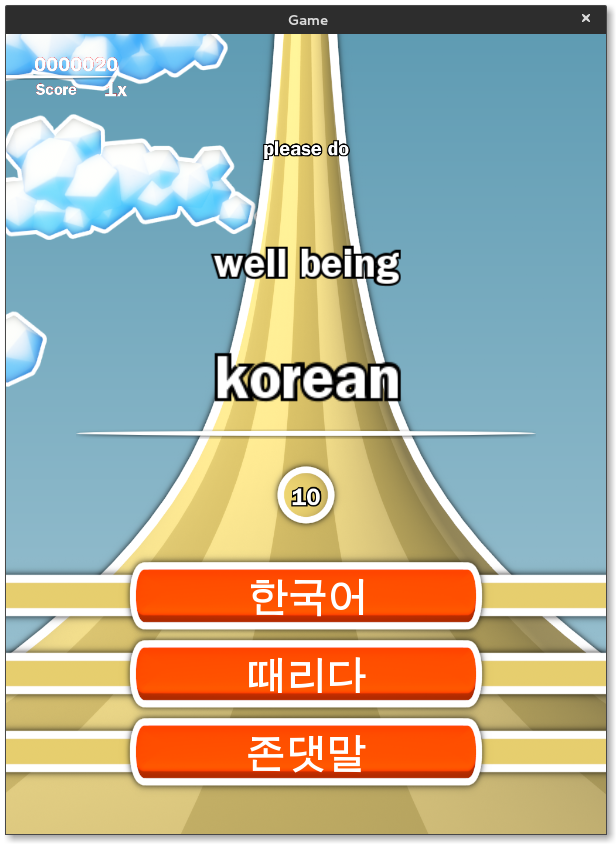
\includegraphics[width=5.5cm]{pic/defg-korean.png}
\end{center}
\caption{Primer delovanja Korejske verzije na namiznem računalniku}
\label{korean}
\end{figure} 


Ena izmed glavnih zahtev igre je izpis različnih pisav in posebnih znakov. Poleg prikazane verzije nemščina angleščina je bila aplikacija razvita tudi z idejo učenja jezikov, ki ne uporabljajo latinice. Slika [\ref{german}] prikazuje primer učenja Korejščine. Aplikacije mora toraj biti sposobna izrisovati velik nabor različnih abeced.

\begin{figure}
\begin{center}
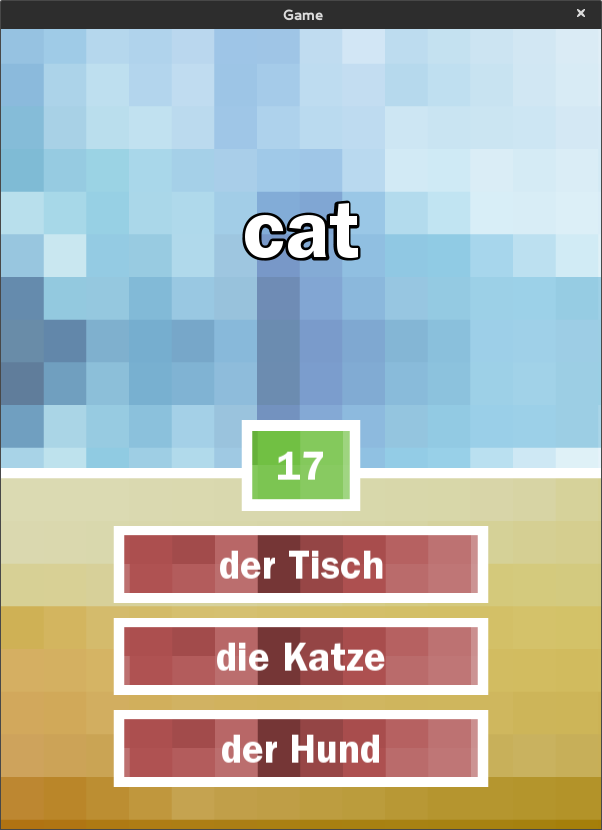
\includegraphics[width=5.5cm]{pic/defg-german.png}
\end{center}
\caption{Primer delovanja Nemške verzije na mobilni napravi}
\label{german}
\end{figure} 

Aplikacija je bila zamišljena kot mobilna aplikacijam za platformi iOS in Android, vendar kot smo že opisali v poglavju[] je zelo uporabno imeti način razvoja na namiznem računalniku.

\subsection{Uporabljena metoda}

Izmed vseh naštetih metod v poglavju[] se nam je zdela najbolj primerna metoda PlayN. Razlogi za izbiro PlayN so naslednji:

\begin{itemize}
\item PlayN je odprtokoden projekt. V primeru težav lahko pogledamo v izvorno kodo projekta in po potrebi nedelovanje spremenimo.
\item Licenca, ki jo PlayN uporablja, ni omejujoča in v primerjavi z nekaterimi plačljivimi metodami, ne zahteva nobenega plačila pred uporabo. To velja tudi, če bi aplikacijo namenili komercialnim namenom.
\item PlayN je še vedno v aktivnem razvoju, razvijalci pa so aktivni na listi za elektronsko pošto (prevod mailing lista).
\item Orodje PlayN omogoča preprosto podporo dodajanje lastnih pisav, kar je ključnega pomena za podporo jezikom kot je Korejščina.
\item Število platform, ki jih PlayN podpira, zadošča potrebam aplikacije.
\item PlayN omogoča uporabo vročega izmenjevanja kode, kar zelo pohitri razvoj aplikacije.
\item Poleg samega ogrodja PlayN je na voljo tudi precej vtičnikov, ki so jih napravili uporabniki. Tak primer je vtičnik Tripleplay, ki je v aplikaciji uporabljen za prikaz menijev.
\item Dokumentacija je dobro napisana in razumljiva.
\end{itemize}

Izbira je potekala med PlayN in podobno knjižnico LibGDX. Na koncu smo se odločili za PlayN zaradi lažje uporabe lastnih pisav v aplikaciji. O uporabi plačljivih rešitev nismo razmišljali.

\subsection{Prednosti izbora metode}



\subsection{Slabosti izbora metode}

Hitrost razvoja bi bil precej lažji, če bi izbrali kakšno od plačljivih rešitev. Z uporabo PlayN smo imeli kar nekaj težav v vzpostavitvi razvijalnega okolja na dveh različnih sistemih - Linux, kjer je potekal glavni razvoj in OSX, ki je bil uporabljen za testiranje iOS verzije.

\section{Unity3D}

Na sliki [\ref{mineditor}] je vidno kako poteka razvoj v okolju Unity.

\begin{figure}
\begin{center}
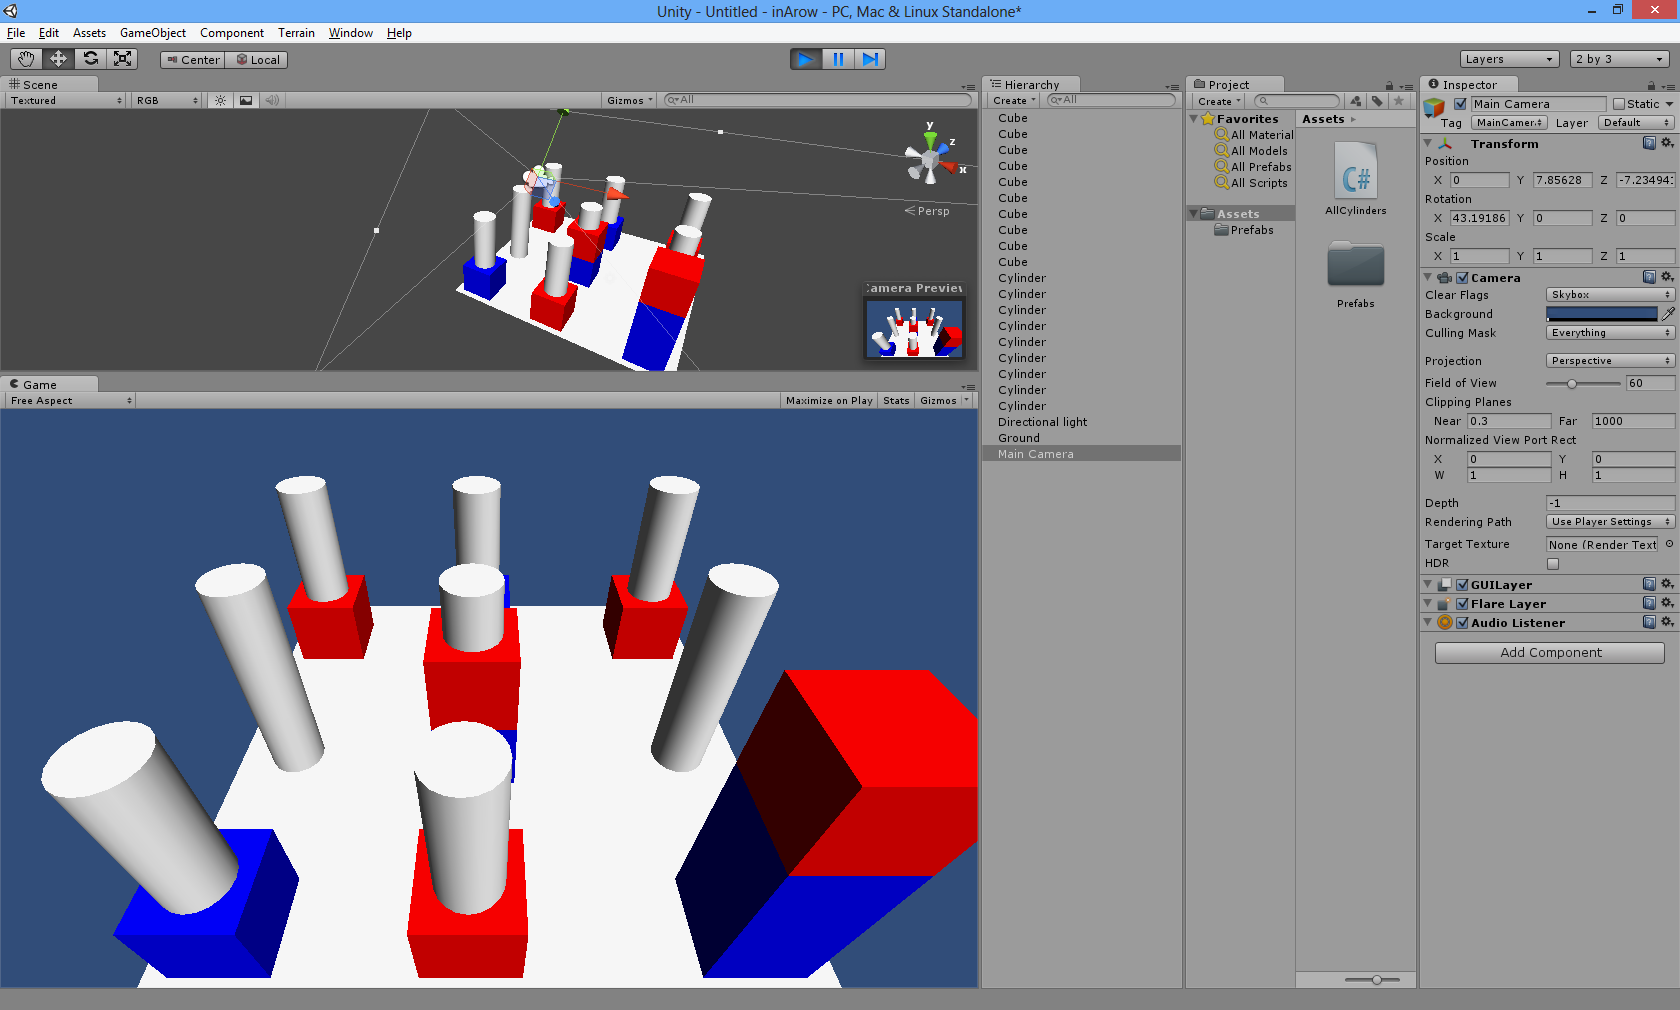
\includegraphics[width=12cm]{pic/min-editor.png}
\end{center}
\caption{Razvoj grafično intenzivne aplikacije v okolju Unity.}
\label{mineditor}
\end{figure} 

Slika \ref{minplay} prikazuje delovanje aplikacije na mobilni platformi Nexus 7.

\begin{figure}
\begin{center}
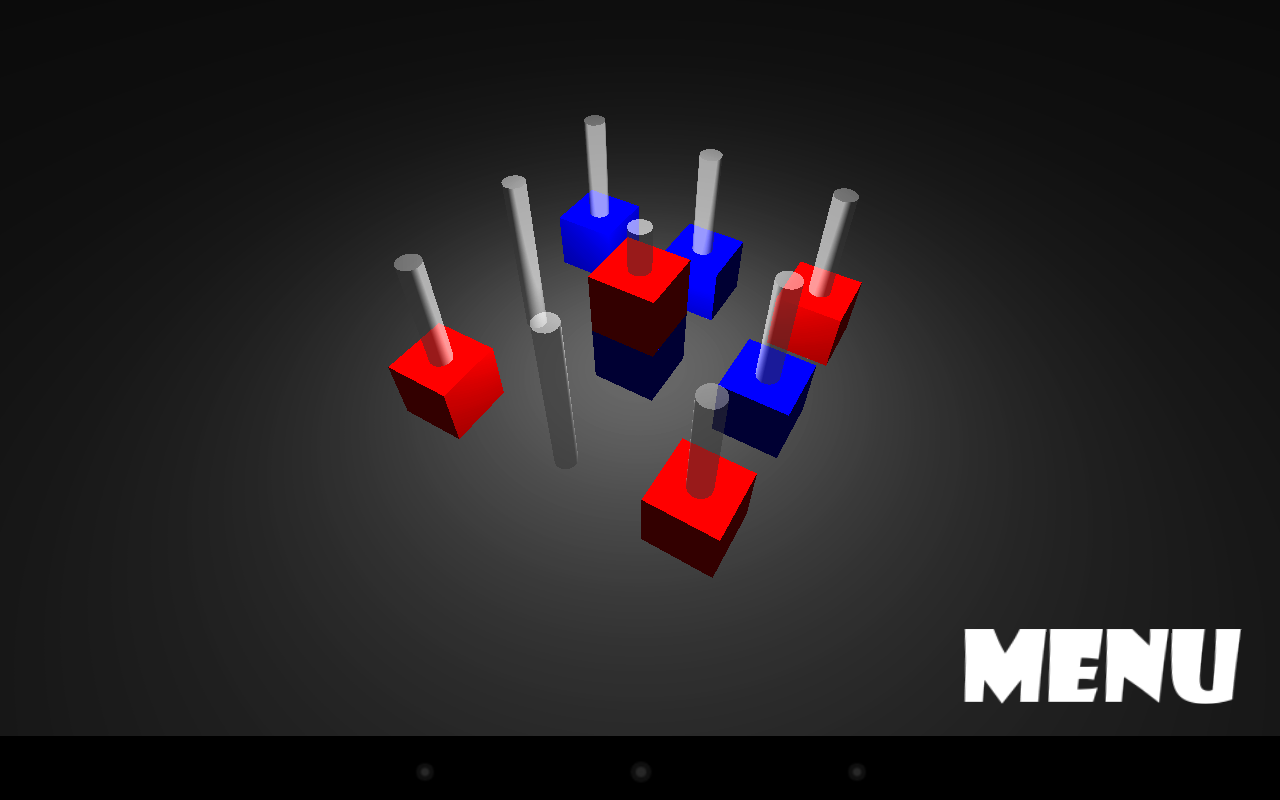
\includegraphics[width=10cm]{pic/min-play.png}
\end{center}
\caption{Končana Unity aplikacija izvožena na mobilno platformo.}
\label{minplay}
\end{figure} 

\section{Primer C++}

%\section{Primer MIN}

%Primer Min je bil narejen s pomočjo knjižnice LibGDX. Za svoje delovanje izrablja %zmoglivosti OpenGL ES 2.0. 


